\section{Computational study and Number of total computations}
\label{sec:plan}

From the subset formalism in Sec.~\ref{sec:bsse_trimer}, the number of
primitive energy evaluations can be expressed compactly. Let $N$ be the
number of monomers. For each fragment size $k$ ($1\le k\le N$), there are
$\binom{N}{k}$ fragments, and each fragment must be evaluated in
$2^{N-k}$ supersets (all subsets that contain it). Thus,
\begin{equation}
N_{\mathrm{eval}}^{\mathrm{all\ terms}}(N)
= \sum_{k=1}^{N} \binom{N}{k}\,2^{\,N-k}.
\label{eq:Neval_all}
\end{equation}

However, when forming the \emph{BSSE} as the difference between the
counterpoise (CP) and standard interaction energies, the $N$-mer total
energy $E_{1\ldots N}(1\ldots N)$ cancels exactly. Therefore, the
$k=N$ term is not required:
\begin{align}
N_{\mathrm{eval}}^{\mathrm{BSSE}}(N)
&= \sum_{k=1}^{N-1} \binom{N}{k}\,2^{\,N-k}
\label{eq:equation-16}
\end{align}
%--
\clearpage
Recalling the binomial theorem\autocite{Beeler2015}, we have that
\[
(x+y)^{n}
  = \sum_{k=0}^{n} \binom{n}{k}\,x^{k}\,y^{\,n-k}.
\]
Thus,
\begin{equation*}
    3^{n}
    = (1+2)^{n}
    = \sum_{k=0}^{n} \binom{n}{k}\,1^{k}\,2^{\,n-k}
    = \sum_{k=0}^{n} \binom{n}{k}\,2^{\,n-k}.
\end{equation*}

\noindent
We can then re-write Eq.~(\ref{eq:equation-16}) by allowing the index
$k$ to range from $0$ to $N$. This defines a sum with $(N+1)$ terms,
that is, two more terms than the original.
These additional terms correspond to the first and last elements of
the full sum and must therefore be subtracted. Hence,
\begin{align*}
\sum_{k=1}^{N-1} \binom{N}{k}\,2^{\,N-k}
&=
\sum_{k=0}^{N} \binom{N}{k}\,2^{\,N-k}
 - \bigl(2^{N} + 1\bigr)
 = 3^{N} - \bigl(2^{N} + 1\bigr),
\end{align*}
where the term $2^{N}$ corresponds to the first term ($k=0$)
and the term $1$ corresponds to the last term ($k=N$).
In this way, we obtain
\begin{align}
N_{\mathrm{eval}}^{\mathrm{BSSE}}(N)
   = 3^{N} - \bigl(2^{N} + 1\bigr).
\label{eq:equation-18}
\end{align}

\noindent\textbf{For the trimer case ($N=3$)}, we have
\[
N_{\mathrm{eval}}^{\mathrm{BSSE}}(3)
= 3^{3} - 2^{3} - 1
= 27 - 8 - 1
= \boxed{18}.
\]
These 18 terms consist of:
\begin{itemize}[leftmargin=2em,topsep=-0.25cm]
  \item $12$ monomer-in-subset energies: each monomer appears in $2^{3-1}=4$ subsets,
        giving $3\times 4 = 12$;
  \item $6$ dimer-in-subset energies: each dimer appears in $2^{3-2}=2$ subsets,
        giving $3\times 2 = 6$.
\end{itemize}
If, in addition, one wishes to report the \emph{counterpoise (CP)},
the trimer total energy $E_{ABC}(ABC)$ must be included:
\[
N_{\mathrm{eval}}^{\mathrm{all\ terms}}(3)
= 18 + 1 = \boxed{19}.
\]

%--
\clearpage
%---
\subsection{Geometry sampling and scaling protocol}
\label{sec:families}

Each \emph{configuration} (geometry/scale) requires the counts above. 
Only the three isolated-monomer energies $E_A(A)$, $E_B(B)$, $E_C(C)$ 
are geometry independent and can be computed once per method/basis.

Hence, with $N_{\mathrm{geom}}$ geometries,
\[
\boxed{
\begin{aligned}
N_{\mathrm{runs}}^{\mathrm{BSSE}}(3)
  &= 3 \;+\; N_{\mathrm{geom}}\,[\,18-3\,]
   \;=\; 3 + 15\,N_{\mathrm{geom}},\\[4pt]
N_{\mathrm{runs}}^{\mathrm{all\ terms}}(3)
  &= 3 \;+\; N_{\mathrm{geom}}\,[\,19-3\,]
   \;=\; 3 + 16\,N_{\mathrm{geom}}.
\end{aligned}}
\]

In the trimer study we consider four shape families:
\emph{linear}, \emph{equilateral}, \emph{isosceles}, and \emph{scalene}
(Fig.~\ref{fig:figure-1}). 
For each family we sample $12$ similar (uniformly scaled) geometries, so
\[
N_{\mathrm{geom}} = 4 \times 12 = 48.
\]
Therefore,
\[
\boxed{
\begin{aligned}
N_{\mathrm{runs}}^{\mathrm{BSSE}}(3) 
  &= 3 + 15\times 48 \;=\; \mathbf{723},\\[2pt]
N_{\mathrm{runs}}^{\mathrm{all\ terms}}(3) 
  &= 3 + 16\times 48 \;=\; \mathbf{771}.
\end{aligned}}
\]

\begin{figure}[!ht]
  \centering
  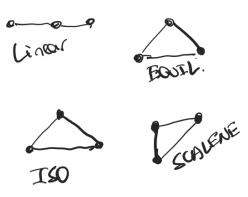
\includegraphics[width=0.28\linewidth]{images/trimers.png}
  \caption{Trimer shape families used for scaling: linear, equilateral, isosceles, and scalene.}
  \label{fig:figure-1}
\end{figure}

\subsection*{\centering Electronic-structure methods and basis sets}

All computations will be performed with three methods
(HF, MP2, CCSD(T)) and two basis sets
(aug-cc-pVDZ, aug-cc-pVTZ). If wall-time permits,
aug-cc-pVQZ will also be included. So, for $M=3$ (methods) and $B\in\{2,3\}$ (basis sets).
The total number of runs is
\[
\boxed{
\begin{aligned}
N_{\mathrm{runs}}^{\mathrm{BSSE}}(3; M,B)
  &= \bigl(3 + 15\,N_{\mathrm{geom}}\bigr)\; M B
   \;=\; \mathbf{723}\; M B,\\[4pt]
N_{\mathrm{runs}}^{\mathrm{all\ terms}}(3; M,B)
  &= \bigl(3 + 16\,N_{\mathrm{geom}}\bigr)\; M B
   \;=\; \mathbf{771}\; M B,
\end{aligned}}
\]
where $N_{\mathrm{geom}}=48$ for the four shape families
with 12 scale points each.

\noindent\textbf{With two basis sets ($B=2$):}
\[
\boxed{
\begin{aligned}
N_{\mathrm{runs}}^{\mathrm{BSSE}}(3)
  &= 723 \times 3 \times 2 = \mathbf{4338},\\[2pt]
N_{\mathrm{runs}}^{\mathrm{all\ terms}}(3)
  &= 771 \times 3 \times 2 = \mathbf{4626}.
\end{aligned}}
\]

\noindent\textbf{If aug-cc-pVQZ is added ($B=3$):}
\[
\boxed{
\begin{aligned}
N_{\mathrm{runs}}^{\mathrm{BSSE}}(3)
  &= 723 \times 3 \times 3 = \mathbf{6507},\\[2pt]
N_{\mathrm{runs}}^{\mathrm{all\ terms}}(3)
  &= 771 \times 3 \times 3 = \mathbf{6939}.
\end{aligned}}
\]


